\section{Results: What History Reads in the Macro Cell}
\label{sec:results-mechanism}

In this section, we identify which part of the macro-cell input carries the history gain of Section~\ref{subsec:gain-macro}, and what that part contains. All comparisons share the samples and user splits of the full $h=5$ input, so each comparison is paired.

% src: followup_2026_10/uniform_nlos/history_mechanism_followup_summary.json summary.{xgboost,random_forest}.{angle_hist,rss_hist,ray_hist,full}.multi.gain_vs_snap.all (20 seeds, Student-t: angle 3.16 +- 0.14 / 3.06 +- 0.13; full 3.15 +- 0.12 / 2.75 +- 0.08; rss 0.23 +- 0.09 / -0.22 +- 0.11; ray 0.25 +- 0.11 / -0.01 +- 0.10); diagnostics_2026_10/baseline_uniform_nlos (k-NN, five seeds: angle 5.19, full 3.79, rss -2.27); diagnostics_2026_10/mixed_propagation (angle-only 2.4-3.6 m, three models); followup_2026_10/neural_uniform_nlos (five seeds: angle_hist 3.11/3.43/3.27/2.98; full 3.07/3.19/3.19/2.85; rss_hist 0.17/0.19/0.16/0.16)
\noindent\textbf{The angle channels.} The test feeds a model history for one group of channels at a time while holding every other channel at its current value: the RSS group~(RSS, SINR and the RSS difference), the angle group~(the sines and cosines of both angles and the azimuth difference), or the ray group~(the two ray-projection coordinates and their differences). For multi-antenna devices on the uniform-NLOS data, angle history alone gives as much as history on every channel, over $20$ splits $3.16$ against \SI{3.15}{\meter} for XGBoost and $3.06$ against \SI{2.75}{\meter} for Random Forest, whereas RSS history and ray history give at most \SI{0.25}{\meter}~(Figure~\ref{fig:angle-decomposition}). The same holds for the other five families over five splits: for $k$-NN angle history alone outperforms the full window, because the RSS lags, which alone raise its error, add noise to its distance metric, and for the four neural models angle history alone lowers the error by $3.0$ to \SI{3.4}{\meter} and RSS history by under \SI{0.2}{\meter}. The mixed-propagation data repeat the pattern. The result therefore covers all seven model families.

% src: followup_2026_10/uniform_nlos summary.xgboost.{snap,full}.multi.shape (20 seeds: radial 17.21 -> 14.06, tangential 4.96 -> 4.61; RF 17.39 -> 14.77, 4.65 -> 4.15); summary.{xgboost,random_forest}.pure_snap.multi.gain_vs_snap.all (20 seeds: -0.56 +- 0.16 / -0.37 +- 0.08)
What the angle history improves is mainly the estimate of distance. For multi-antenna devices, five steps of history lowered XGBoost's mean radial error from $17.2$ to \SI{14.1}{\meter} but its tangential error only from $5.0$ to \SI{4.6}{\meter}, and Random Forest behaves alike; bearing is already well determined by the current angle, and the window improves range. It should be noted that the $h=0$ input already holds one step of change through its first differences: removing them raises the multi-antenna error by \SI{0.56}{\meter} for XGBoost and \SI{0.37}{\meter} for Random Forest, so the gains reported here understate the full effect of history by roughly \SI{15}{\percent}.

\subsection{What the Angle History Contains}
\label{subsec:averaging}

% src: followup_2026_10/uniform_nlos (20 seeds, XGBoost / RF, multi-antenna, Student-t): full 3.15+-0.12 / 2.75+-0.08; angle_hist 3.16+-0.14 / 3.06+-0.13; angle_mean 3.38+-0.19 / 3.61+-0.19; angle_shuffled 2.93+-0.12 / 2.66+-0.13; el_hist 2.72+-0.13 / 2.24+-0.12; az_hist 0.63+-0.08 / 0.77+-0.05
Section~\ref{subsec:history-dof} sets out two ways in which a window of angles can carry position: through its rate of change, since for a given sideways movement the bearing turns at the rate $v_\perp/r$, or through repeated noisy samples, since every angle report is the true angle plus an independent \ang{4} error quantized to \ang{5} steps, and averaging several reports of a nearly unchanged angle gives a better estimate. Four tests over $20$ splits separate the two~(Figure~\ref{fig:angle-decomposition}): (i)~replacing the window by the unordered mean of each angle channel gives as much as the ordered history; (ii)~shuffling the order of the earlier reports costs only $0.2$ to \SI{0.4}{\meter}; (iii)~elevation history alone gives most of the gain; and (iv)~azimuth history alone gives under \SI{0.8}{\meter}. The BS stands about \SI{8.5}{\meter} above a device, so elevation encodes distance, and averaging it improves the range estimate; this is why it is the radial error that falls with history.

\begin{figure}[h]
  \centering
  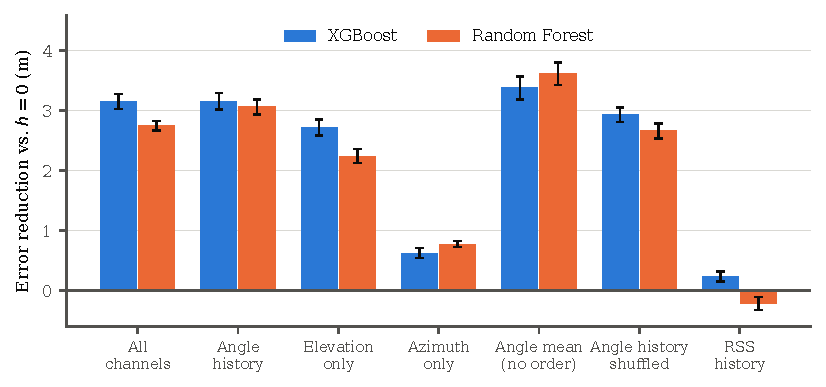
\includegraphics[width=0.95\textwidth]{fig_angle_decomposition}
  \caption{Macro cell, uniform NLOS: reduction in multi-antenna error from $h=0$ to $h=5$ when history is given for all channels, parts of the angle information, or RSS only. Seed-paired means over $20$ user splits with \SI{95}{\percent} Student-$t$ intervals.}
  \label{fig:angle-decomposition}
\end{figure}
% src: figure_scripts/python/make_figures_followup.py angle_decomposition()

% src: followup_2026_10/aoa_impairment/{clean,quant5_only,noise4_only,noise8_quant5} (10 seeds, full history, multi-antenna; clean: XGB h=0 2.32 m, RF 1.58 m, gain +0.00 +- 0.11 / -1.02 +- 0.03; quantization only: h=0 14.2 m, gain 1.9 / 2.3 m; noise only 3.1 m); neural_exact_aoa (gain -0.48 to -0.78 m; h=0 error 1.8-3.2 m)
The decisive test removes the error. With exact arrival angles the multi-antenna error without history falls to between $1.6$ and \SI{3.2}{\meter} across the six models tested, and history adds nothing for XGBoost and makes Random Forest and the four neural models worse: there is nothing left to average. Quantization alone, or noise alone, still leaves a gain~(Figure~\ref{fig:aoa-error-model}a). The history gain of Section~\ref{subsec:gain-macro} is thus a property of averaging imperfect angle reports, not of bearing geometry.

\begin{figure}[h]
  \centering
  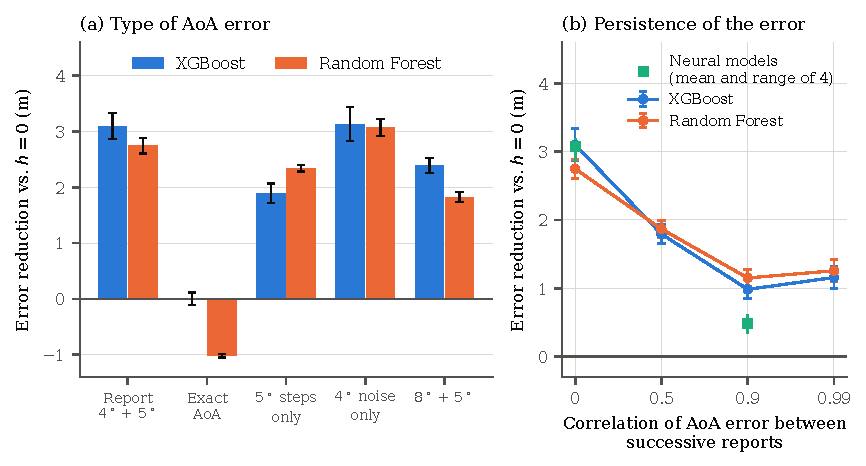
\includegraphics[width=0.95\textwidth]{fig_aoa_error_model}
  \caption{Macro cell, uniform NLOS: reduction in multi-antenna error from $h=0$ to $h=5$ under (a)~different types of angle error and (b)~a \ang{4} error correlated between successive reports. Ten user splits per point, five for the neural models; \SI{95}{\percent} Student-$t$ intervals.}
  \label{fig:aoa-error-model}
\end{figure}
% src: figure_scripts/python/make_figures_followup.py aoa_error_model()

% src: followup_2026_10/aoa_impairment/corr_rho{0,0.5,0.9,0.99} (10 seeds; XGB full +3.10, +1.79, +0.98, +1.16; elevation +2.69 -> +0.03; RF +2.75 -> +1.26); neural_corr_rho0.9 (+0.34 to +0.61 m, 2-3 %)
How much of the gain remains depends on how the error behaves from one report to the next. If the angle error persists across the window, averaging cannot remove it. Making the \ang{4} error an autoregressive sequence along each walk, XGBoost's gain falls from \SI{3.1}{\meter} with independent errors to about \SI{1}{\meter} at lag-1 correlations of $0.9$ and above~(Figure~\ref{fig:aoa-error-model}b). The elevation part disappears first; what remains, $5$ to \SI{7}{\percent} of the error, is in azimuth, and the neural models keep only $2$ to \SI{3}{\percent}. The headline gain of $15$ to \SI{21}{\percent} is therefore specific to angle errors that are independent between reports, which is how the macro-cell simulation draws them.

% src: followup_2026_10/history_depth/h{1,3,10,20} (10 seeds) and uniform_nlos (h=5, 20 seeds), XGBoost multi-antenna full +1.21, +2.53, +3.15, +3.51, +3.68; angle_mean +1.26, +2.72, +3.38, +3.16, +1.39; angle_hist at h=20 +3.59
The same account explains how the gain depends on window length. The unordered mean of the angle window is the better input up to five steps and then fails, falling to \SI{1.4}{\meter} at twenty steps, because over \SI{80}{\meter} of travel the true angle has changed and an unweighted mean is biased; the ordered window still gives \SI{3.6}{\meter} there, since the model can weight recent reports. At long windows the order of the reports does matter in the macro cell, for discounting stale ones.
